\newpage
\section{Comparison and Discussion}

The pretrained MuRIL model demonstrates a clear advantage over the classical machine learning pipeline. On raw tweets, plain MuRIL achieves a test macro-F1 of 0.606, comfortably outperforming the TF-IDF + Random Forest baseline (0.583) by over 2.3 points. 

\begin{figure}[H]
    \centering
    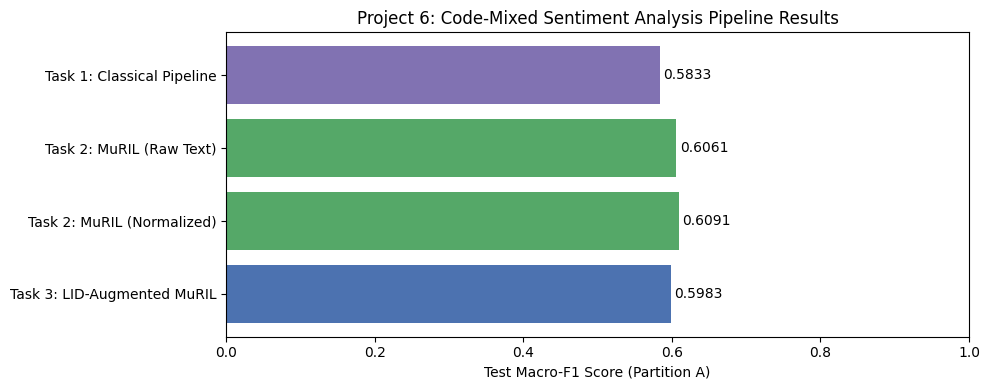
\includegraphics[width=0.9\textwidth]{final_comparison.png}
    \caption{Test macro-F1 of all four systems on the 616 Partition A test tweets.}
    \label{fig:final_comparison}
\end{figure}

\subsection*{What the tasks asked}
\begin{itemize}
    \item \textbf{How much of Task 1's normalization does MuRIL absorb on its own?} Nearly all of it. MuRIL beats Task 1 even when processing completely raw, unnormalized text. Interestingly, applying the Dakshina normalization at test time yielded a marginal improvement (from 0.606 to 0.609). This suggests that while MuRIL's subword tokenizer handles most spelling variations robustly on its own, standardizing certain highly irregular code-mixed tokens at inference can still provide a tiny benefit without disrupting the learned representations.
    
    \item \textbf{Are LID and MuRIL complementary?} Not clearly, at least on our specific partition. The LID-augmented model (Task 3) achieved a macro-F1 of 0.598. While this remains superior to the classical baseline, it falls slightly below plain MuRIL (0.606). Given the test set size of only 616 tweets, a gap of this size ($\sim$0.008) is well within the margin of random chance. The lack of significant improvement suggests that MuRIL's deep layers can already distinguish between Hindi and English implicitly based on subword patterns, rendering the explicit Task 1 tags somewhat redundant.
\end{itemize}

\subsection*{Limitations}
\begin{itemize}
    \item \textbf{Sample Size and Variance:} With only 616 test tweets and a single training run per system, minor metric differences (under 1--2 points) may be attributable to initialization and sampling chance rather than true architectural superiority.
    \item \textbf{Lexicon Constraints:} The Dakshina lexicon is a 30,000-word sample. Relying strictly on the ``most frequent spelling'' rule forces some incorrect deterministic mappings, which can degrade the input quality for both Task 1 and Task 3.
    \item \textbf{Emoji Handling:} MuRIL tokenizes emojis as \texttt{[UNK]}. Code-mixed social media text heavily relies on emojis for sentiment expression, meaning all MuRIL-based tasks drop a highly predictive source of sentiment signal.
\end{itemize}